\documentclass[conference]{IEEEtran}
\IEEEoverridecommandlockouts
% The preceding line is only needed to identify funding in the first footnote. If that is unneeded, please comment it out.
\usepackage{cite}
\usepackage{amsmath,amssymb,amsfonts}
\usepackage{algorithmic}
\usepackage{graphicx}
\graphicspath{ {images/} }
\usepackage{textcomp}
\usepackage{xcolor}
\usepackage{stackengine}
\stackMath
\def\BibTeX{{\rm B\kern-.05em{\sc i\kern-.025em b}\kern-.08em
    T\kern-.1667em\lower.7ex\hbox{E}\kern-.125emX}}
\begin{document}

\title{Resource Access Protocols\\
{\footnotesize }
\thanks{Identify applicable funding agency here. If none, delete this.}
}

\author{\IEEEauthorblockN{1\textsuperscript{st} Sheikh Muhammad Adib Bin Sh Abu Bakar}
\IEEEauthorblockA{\textit{Hochshule Hamm-Lippstadt} \\
\textit{B.Eng. Electronic Engineering}\\
Lippstadt, Germany \\
sheikh-muhammad-adib.bin-sh-abu-bakar@stud.hshl.de}

}

\maketitle
\begin{abstract}

In hard real time system, it is important to ensure every single task not only to be successfully executed but to produce the right value on the right time. Thus, scheduling algorithm play a big role in handling various of task, either statically or dynamically. It is common in real time system environment, some tasks share the same resource, which is one of the complicated part in concurrent operating system. Any concurrent operating system should utilize proper synchronization to assure mutual exclusion among competing activities, in order to ensure the predictability of the system, which is important in oder to produce reliable system especially when safety is a crucial part. This is why resource access protocol one of the important topic in building a real time system. In this research paper, various of resource access protocol for uni-processor that are developed under fixed priority assignment will be explained. So, it will be clear for us which protocol should be implemented based on the environment that we are working on. To ensure this paper is easy to understand, I also include basic information about real time system before going deep into resource access protocol.
\end{abstract}



\begin{IEEEkeywords}
real time system, resource, protocol 
\end{IEEEkeywords}

\subsection{Real Time System}


\subsection{Characteristics}

%Real Time System
%predictibility

%task
%scheduling
%classification
%-preemtion
%-non-preemtion
%-dynamic
%-static
%-online
%periodic
%constraint
%-timming
%-resource
%schedubility test

\section{Task Scheduling}
In this section we will describe the concept and terms that are dominant in this research paper.

\subsection{Task, Job, Thread and Process}

Task, thread, job and process  are the basic building block in task scheduling. Their definition are listed below according to \cite{b4}

\begin{itemize}
\item Task: a sequence of instructions that, in the absence of other activities, is continuously executed by the processor until completion.
\item Job: an instance of a task executed on a specific input data.
\item Thread: a task sharing a common memory space with other tasks.
\item Process: a task with its private memory space, potentially generating different threads sharing the same memory space.
\end{itemize}


\subsection{Scheduling Policy and Scheduling Algorithm }

When a single processor has to execute a set of concurrent tasks – that is, tasks that can overlap in time – the CPU has to be assigned to the various tasks according to a predefined criterion, called a scheduling policy and the set of rules that, at any time, determines the order in which tasks are executed is called a scheduling algorithm \cite{b5}.

Considering that the schedule algorithm handles more than one task, now we will extend the definition of a task correspond to their state according to \cite{b5}

\begin{itemize}
\item A task that could potentially execute on the CPU can be either in execution (if it has been selected by the scheduling algorithm) or waiting for the CPU (if another task is executing).

\item A task that can potentially execute on the processor, independently on its actual availability, is called an active task.

\item A task waiting for the processor is called a ready task, whereas the task in execution is called a running task.

\item All ready tasks waiting for the processor are kept in a queue, called ready queue.

\end{itemize}

\subsection{Classification of Scheduling Algorithms}

In this subtopic we will only focus on important classification of scheduling algorithm that are related to the scope of this research paper. 

\begin{itemize}
\item Preemptive: running task can be interrupted at any time.
\item Non-preemptive: a task, once started is executed until completion
\item Static: scheduling decisions are based on fixed parameters (off-line) .
\item Dynamic: scheduling decisions are based on parameters that change during system evolution.
\item Off-line : Scheduling algorithm is performed on the entire task set before start of system. Calculated schedule is executed by dispatcher. 
\item On-line : scheduling decisions are taken at run-time every time a task enters or leaves the system.
\item Optimal : the algorithm minimizes some given cost function, alternatively : it may fail to meet a deadline only if no other algorithm of the same class can meet it.
\item Heuristic : algorithm that tends to find the optimal schedule but does not guarantee to find it

\end{itemize}


\subsection{Periodic and Aperiodic Task}

A task can be periodic or aperiodic base on the way it is activated. Their definition are listed below according to \cite{b4}
\begin{itemize}
\item Periodic Task: a task in which jobs are activated at regular intervals of time, such that the activation of consecutive jobs is separated by a fixed interval of time, called the task period.
\item Aperiodic Task: a task in which jobs may be activated at arbitrary time intervals.
\end{itemize}

The topic of this paper is limited to periodic tasks. Figure \ref{fig:periodic} shows an example of periodic task.

\begin{figure}[h]
    \centering
    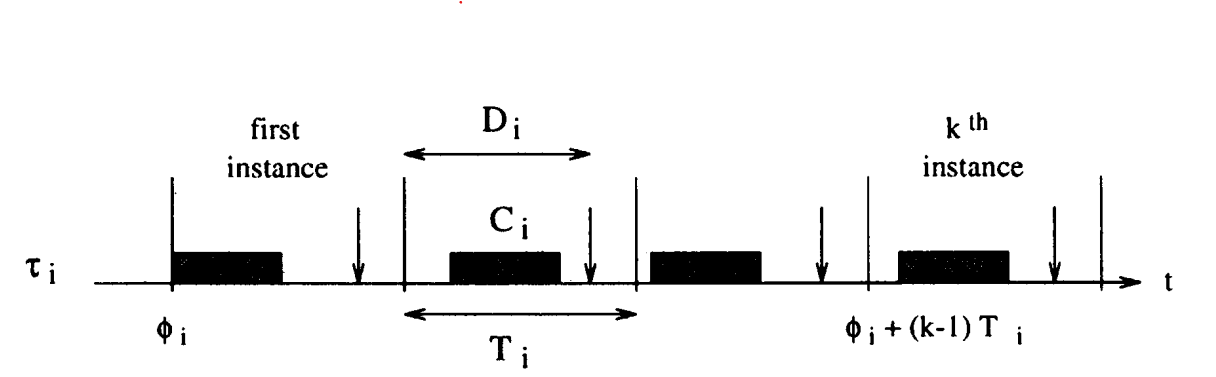
\includegraphics[width=0.5\textwidth]{periodic}
    \caption{periodic task \cite{b5}}
    \label{fig:periodic}
\end{figure}

\subsection{Type of task constraint}

Task constraints are used by the scheduling algorithm to set  priority for each task. There are 3 main type of task constraint and they are:

\begin{itemize}
\item Timing constraint
\item Precedence constraint
\item Resource constraint
\end{itemize}

Next we will explain more detail about timing constraint and resource constraint. Precedence constraint is not covered in this paper. 

\subsubsection{Timing Constraint}

One of the timing constraint that are essential in this paper is deadline. There is two type of deadline:
\begin{itemize}
\item Relative Deadline: the longest interval of time within which any job should complete its execution\cite{b4}.
\item Absolute Deadline (of a job): the time at which a specific job should complete its execution\cite{b4}.
\end{itemize}

With time constraint we can characterize real time system into three category :
\begin{itemize}
\item Hard Real Time System - failed to met the deadline can cause catastrophic event 
\item Soft Real Time System - failed to met the deadline only cause the degradation of the system 
\item Firm Real Time System - failed to met the deadline only cause the production of useless output 
\end{itemize}

Hard real time is the main focus in this research paper.
\subsubsection{Resource Constraint}

Another important constraint related to this topic is resource constraint. 

According to \cite{b5} - resource is any software structure that can be used by the process to advance its execution. Typically, a resource can be a data structure, a set of variables, a main memory area, a file, a piece of program, or a set of registers of a peripheral device. A resource dedicated to a particular process is said to be private, whereas a resource that can be used by more tasks is called a shared resource.

Many shared resources do not allow concurrent access by competing processes in order to ensure data consistency, and instead require mutual exclusion. This means that if another task is within R modifying its data structures, a task cannot access R. R is referred to as a mutually exclusive resource in this scenario.  A piece of code executed under mutual exclusion constraints is called a critical section. This can be illustrate in figure \ref{fig:Two_tasks_sharing} where R is the mutually exclusive resource, $ \tau_{1} $ and $\tau_{2} $ are two distinct task.

In figure \ref{fig:Example_of_schedule_creating_data_inconsistency} we can see the data inconsistency without mutual exclusion
\begin{figure}[h]
    \centering
    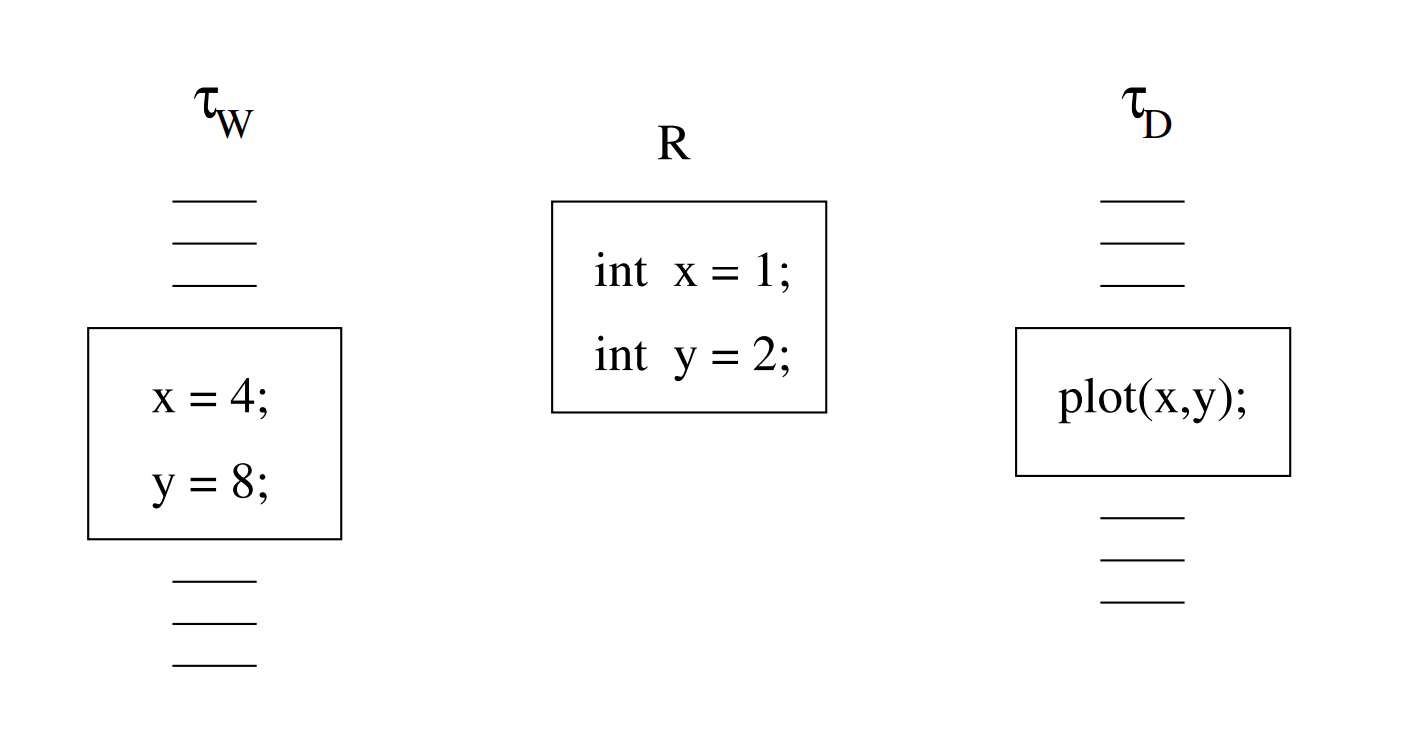
\includegraphics[width=0.5\textwidth]{Two_tasks_sharing}
    \caption{ Two tasks sharing a buffer with two variables. \cite{b5}}
    \label{fig:Two_tasks_sharing}
\end{figure}

\begin{figure}[h]
    \centering
    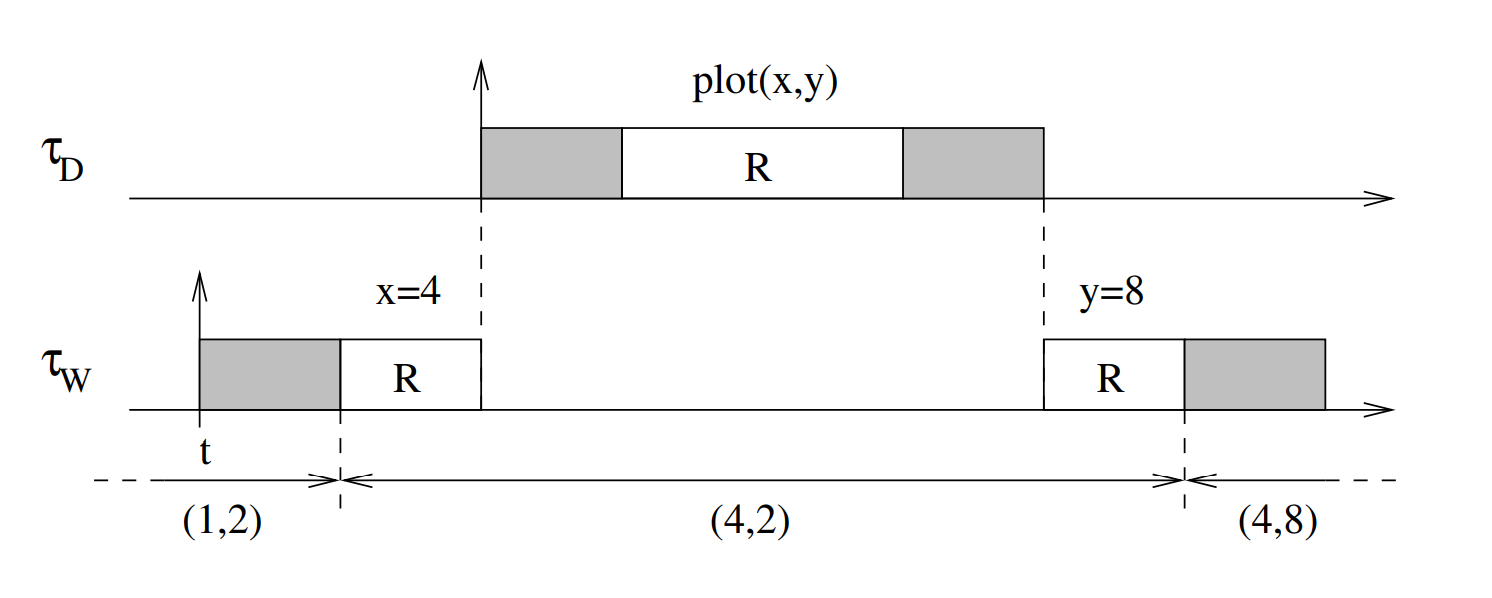
\includegraphics[width=0.5\textwidth]{Example_of_schedule_creating_data_inconsistency}
    \caption{Example of schedule creating data inconsistency. \cite{b5}}
    \label{fig:Example_of_schedule_creating_data_inconsistency}
\end{figure}

Semaphore is one of the very well known example of mechanism for synchronization provided by operating system. Each critical section must begin with wait(S) primitive and end with signal(s) primitive where s is a binary semaphore as shown in figure \ref{fig:Structure}. If a task want to access a resource that currently accessed by another task, that task must wait until signal(S) is executed by the previous task as illustrated in figure \ref{fig:semaphore} and the states of the task are shown in figure \ref{fig:state}

\begin{figure}[h]
    \centering
    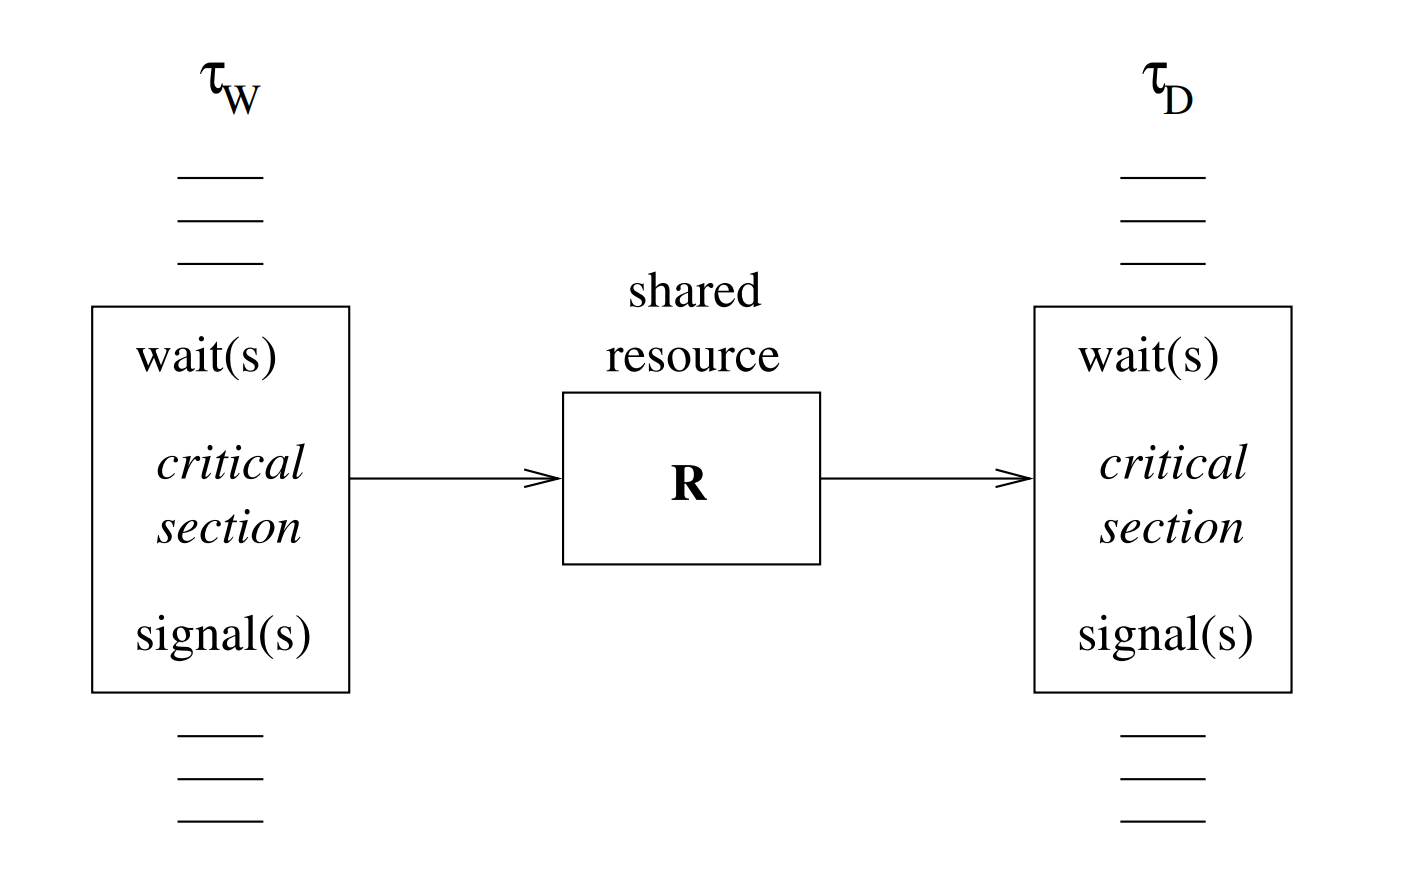
\includegraphics[width=0.5\textwidth]{Structure}
    \caption{Structure of two tasks that share a mutually exclusive resource protected by
a semaphore. \cite{b5}}
    \label{fig:Structure}
\end{figure}

\begin{figure}[h]
    \centering
    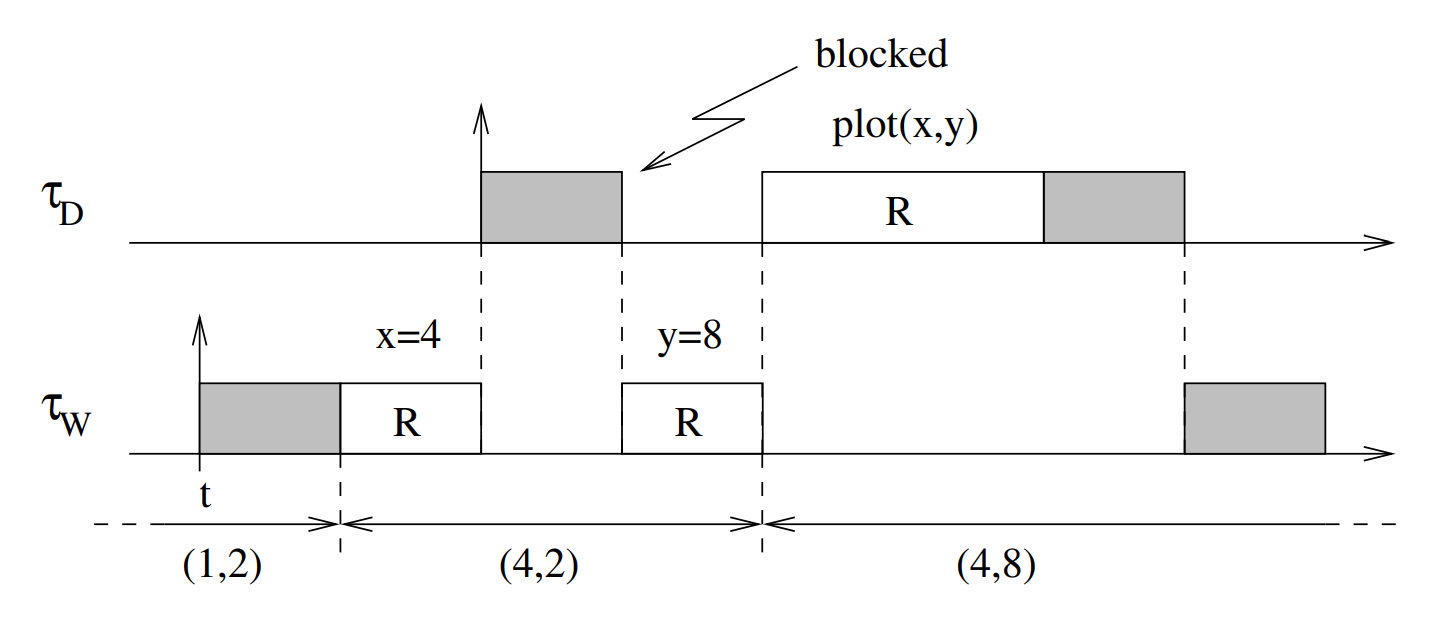
\includegraphics[width=0.5\textwidth]{semaphore}
    \caption{Example of schedule when the resource is protected by a semaphore.. \cite{b5}}
    \label{fig:semaphore}
\end{figure}

\begin{figure}[h]
    \centering
    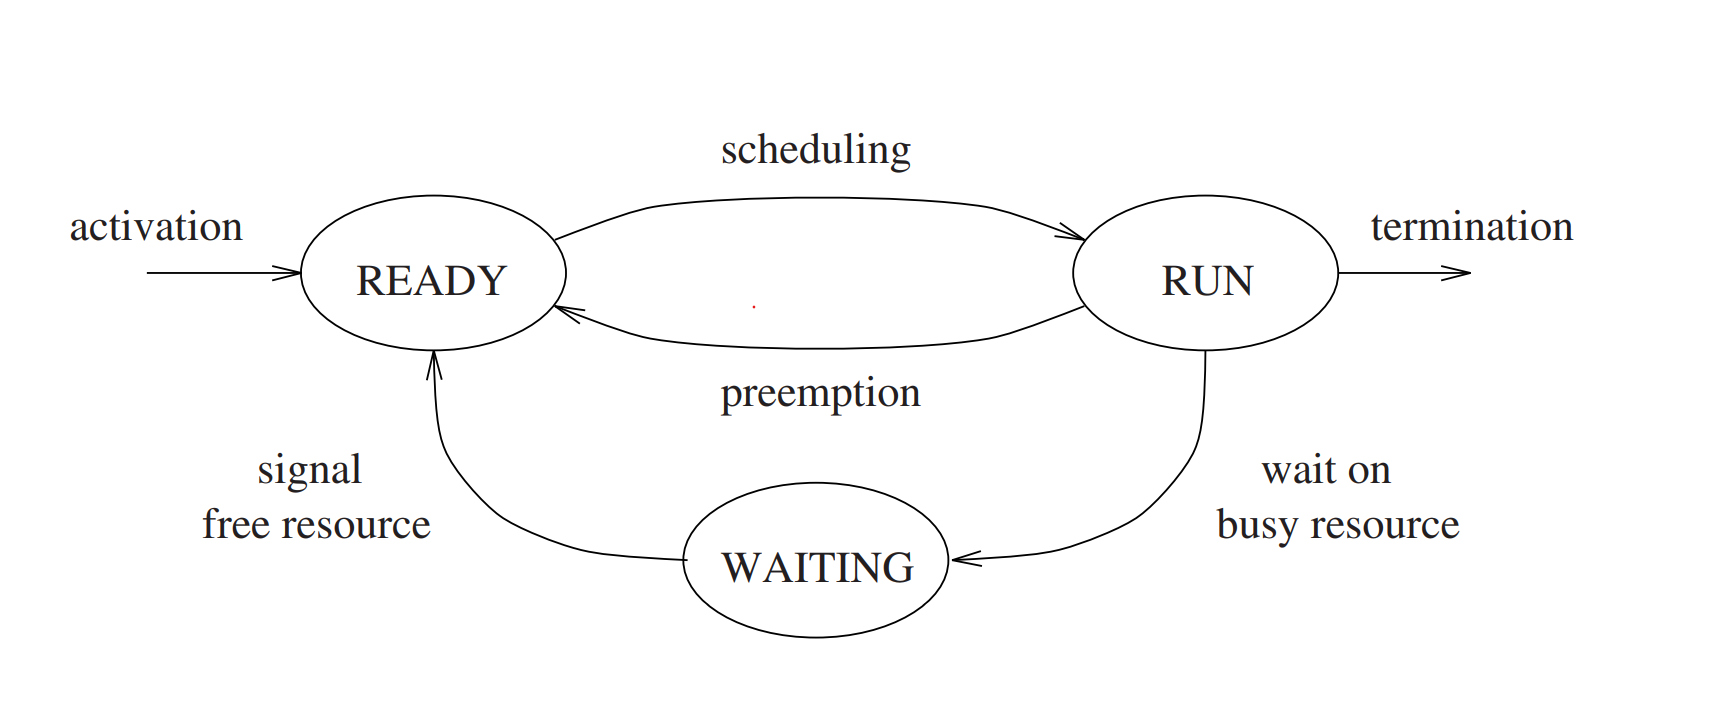
\includegraphics[width=0.5\textwidth]{state}
    \caption{Waiting state caused by resource constraints. \cite{b5}}
    \label{fig:state}
\end{figure}



\subsection{Schedulability}

Before we considering to implement resource access protocol it is important to make sure that all task are schedulable or a schedule is feasible on the set of task. This can be done through scheduability test. This paper will not explain about scheduability test since all task already considered as schedulable. More detail about scheduability test can be found in \cite{b5}.






%task
%scheduling
%classification
%-preemtion
%-non-preemtion
%-dynamic
%-static
%-online
%periodic
%constraint
%-timming
%-resource
%schedubility test

\section{Problem Definition: Invention Priority}

In theory, a set of task that are schedulable will be executed upon on its arriving time and preempted if a task with higher priority arrive. That will not be always true if we apply resource constraint. The problem arrive when a scheduler want to preempt a lower task that is currently accessing a  resource, R and want to execute higher priority task that also want to use the resource. Since the lower priority task didn't yet produce signal(S) primitive where S is the binary semaphore, the higher priority task will be blocked. This phenomenon called priority invention. The implication from this phenomenon is that it will cause unbounded delay on execution of task with higher priority and reduce the predictability of the system because the highest priority task could miss its deadline. The priority invention is illustrated in figure \ref{fig:Example_in_which_NPP_causes_unnecessary_blocking_on_T1} where $ \tau_{1} $ have the highest priority.

Here is where we need resource access protocol to make some adjustment to the scheduler so that the implication of invention priority could be reduced. We're going to discuss this solution in the next sections.
%protocol invention


\subsection{Introduction}
\subsection{Model Classification}
\subsection{Terminology and Assumption}
%Introduction
%Model Classification
%Terminology and Assumption

\section{Compare}

\section{Conclusion}

\section*{Acknowledgment}

I, Sheikh Muhammad Adib 

\begin{thebibliography}{00}

\bibitem{b1}"IEEE Standard for a Real-Time Operating System (RTOS) for Small-Scale Embedded Systems," in IEEE Std 2050-2018 , vol., no., pp.1-333, 24 Aug. 2018, doi: 10.1109/IEEESTD.2018.8445674.

\bibitem{b2} “Real-time systems overview and examples,” Intel. [Online]. Available: https://www.intel.com/content/www/us/en/robotics/real-time-systems.html. [Accessed: 04-May-2022]. 

\bibitem{b3}“Characteristics of real-time systems,” GeeksforGeeks, 04-May-2020. [Online]. Available: https://www.geeksforgeeks.org/characteristics-of-real-time-systems/. [Accessed: 04-Apr-2022]. 

\bibitem{b4} “Terminology and notation,” Terminology and Notation |. [Online]. Available: https://cmte.ieee.org/tcrts/education/terminology-and-notation/. [Accessed: 04-Apr-2022]. 

\bibitem{b5} G. C. Buttazzo, "Hard real-time computing systems: Predictable scheduling algorithms and applications". New York: Springer, 2011. 

\bibitem{b6} L. Sha, R. Rajkumar and J. P. Lehoczky, "Priority inheritance protocols: an approach to real-time synchronization," in IEEE Transactions on Computers, vol. 39, no. 9, pp. 1175-1185, Sept. 1990, doi: 10.1109/12.57058.

\bibitem{b7} Rajkumar, Raj and Juvva, Kanaka and Molano, Anastasio and Oikawa, Shuichi "Resource Kernels: A Resource-centric Approach to Real-Time and Multimedia Systems" 1997 Proceedings of SPIE - The International Society for Optical Engineering. 3310. 10.1117/12.298417. 

\bibitem{b8} Nakajima, Tatsuo and Tokuda, Hideyuki, "Real-Time Synchronization in Real-Time Mach", 1994 
\end{thebibliography}







\end{document}
